\documentclass [a4paper,11pt]{article}

\usepackage [francais]{babel}
\usepackage[utf8]{inputenc}%       encodage du fichier source
\usepackage[T1]{fontenc}%          gestion des accents (pour les pdf)
\usepackage[a4paper]{geometry}%    taille correcte du papier
\usepackage{hyperref}%			   gestion des hyperliens
\usepackage{graphicx}%			   gestion des images
\usepackage{fancyhdr}%
\usepackage{lastpage}%			   pour avoir le numero de page
\usepackage{fancyvrb}%			   meilleur verbatim
\usepackage{chngcntr}%			   pour numéroté les figures au lieux du numéro de section
\usepackage[toc,page]{appendix}%   pour les annexes

% Chemin par defaut des images
\graphicspath{{img/}}

\pagestyle{fancyplain}
\fancyhf{}
\cfoot{\thepage\ sur \pageref{LastPage}}


\begin{document}

\begin{titlepage}
\begin{center}
{\bf Université Sciences et Technologies - Bordeaux1} \vspace{0.5cm}\\

{\bf {\large Master 2 Informatique : Genie logiciel parcours conduite de projet}}\\
%{\emph{Rapport du Projet d'Etude et de Développement }}\\\vspace{1cm}

\begin{figure}[!ht]
  \centering
  
\includegraphics[scale=0.2]{img/uniBx-logo}

  \label{fig:logUniBx}
\end{figure}


{\large{\bf{Rapport:}}}\\\vspace{1cm}
{\huge{\bf Visualisation interactive de topologie de plates-formes parallèles avec lstopo et HTML}}\\\vspace{0.5cm}





\end{center}

\hspace{1cm}\textbf{Réalisé par:} GreenScrum \\
%\bigskip

\hspace{1cm}\textbf{Encadré par:} Philippe Narbel , David Auber.\\


\hspace{1cm}\textbf{Client:} Brice Goglin\\



\end{titlepage}





\tableofcontents

\newpage

\section{Introduction}

hwloc (Hardware Locality) est une bibliothèque logicielle exposant de manière portable et abstraite la topologie des machines, en terme de coeurs, caches partagés, threads, sockets, noeuds numa … . Elle est notamment utilisée par la plupart des bibliothèques de calcul parallèle de type MPI, OpenMP, … pour maîtriser le matériel et ainsi mieux l'exploiter en tenant compte des affinités entre différents composants et entre composants et tâches de calcul. Le composant le plus célèbre de hwloc est l'outil lstopo qui permet de visualiser dans de nombreux formats la topologie de la plate-forme telle que modélisée par hwloc.
Le projet était composé de 2 parties avec une partie en C et une autre qui utilise les technologies Web. Le but de la 1ère partie devait être de créer une exportation des données à visualiser tandis que la seconde était une visualisation du code html suscité. Après discussion avec le client, nous avons compris que la première partie n'etait pas nécessaire étant donné que le fichier xml en sortie suffisait pour obtenir les données nécessaires à la création de l'application de visualisation. La seconde partie était donc la visualisation des données en ajoutant des options pour une personnalisation du rendu final.

\newpage
\section{Architecture}

\subsection{MVC}
L’image ci-dessous réalisée avec le logiciel Enterprise Architect représente un schéma de l’architecture de l’application. Il est important de comprendre que ce schéma n’utilise pas une norme ni même un langage de modélisation en particulier. Il a simplement été conçu pour simplifier la compréhension et les liens existants entre les différentes entités de l’application, il ne peut être considéré comme exactement conforme à la réalité.
\newline

\begin{figure}[!h]
\centering
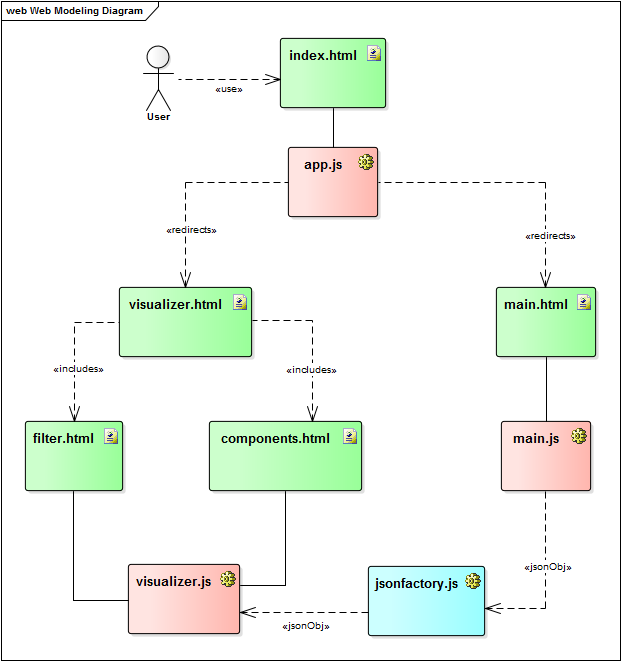
\includegraphics[scale=0.5]{img/ped_architecture.png}
\caption[Résultats]{Architecture simplifiée de l'application}
\end{figure}


D’une certaine façon l’application est organisée suivant une architecture modèle-vue-contrôleur avec quelques particularités. Dans un souci de lisibilité, le schéma utilise un système de couleur. En vert sont représentées les vues qui, dans notre cas, correspondent à des fichiers HTML et en rouge les différents contrôleurs.\newline

\newpage

Lors de la création du site web, nous avions utilisé une architecture \textbf{monopage} (single-page application) avec Angular Js,
c'est à dire une application web accessible via une page web unique, contrairement à un site web classique composés de plusieurs pages
et donc de plusieurs codes sources.\\
Cette architecture nous permet de naviguer sur le site de la même manière qu'un site web classique mais sans avoir à recharger
notre page à chaque action demandée, plus précisément les liens ne rechargent pas la page mais le contenu est modifié au fur
et à mesure selon les requêtes.\\
Pour ce faire il existe deux manières differentes: soit on charge tout les éléments dans un fichier html (template),
soit on récupere et affiche dynamiquement les ressources nécessaires selon les requêtes envoyées par l'utilisateur.\\ \\

  
Avant de rentrer plus en détails, il est nécessaire de faire le point sur les objectifs des différentes entités présents sur le schéma :
\newline

\begin{itemize}
 \item \textbf{index.html} et \textbf{app.js} sont en charge du routage.
 \item \textbf{main.html} et son contrôleur \textbf{main.js} sélectionnent, récupèrent et traduisent les données du fichier XML.
 \item \textbf{visualizer.html}, \textbf{filter.html}, \textbf{components.html} et leur contrôleur visualizer.js affichent et permettent d’interagir avec les données issues du fichier XML.
 \item \textbf{jsonfactory.js} en bleu est un service qui transmet les données issues du fichier XML entre les deux contrôleurs décrits précédemment.
 \newline
\end{itemize}

L’utilisateur accède à l’application via index.html qui est le layout général. Cette page associée au script app.js gère le système de routage de l’application et va insérer le bon template (main.html ou visualizer.html) en fonction de l’URL demandé et en particulier des ancres.
\newline

Dans notre cas, il n’existe pas de choix à proprement parler. Lorsque l’utilisateur lance l’application il est forcément dirigé sur main.html qui est la vue en charge de sélectionner le fichier XML à analyser. Le contrôleur associé main.js va traduire ce fichier XML au format JSON et insérer toutes les informations dans une variable javascript qu’il va transmettre au service jsonfactory.js en vue d’être exploitée par le contrôleur visualizer.js.
\newline

La vue visualizer.html inclus deux fragments externes HTML. Le premier, filter.html décrit l’interface graphique avec les différents boutons et autres éléments sur lesquels l’utilisateur peut interagir. Le second n’est autre que components.html qui est la vue pour l’affichage des informations provenant indirectement du fichier XML.
\newline

Ces vues sont en relation avec le script visualizer.js qui contient deux contrôleurs. Le premier contient plusieurs types de fonctions :
\newline

\begin{itemize}
 \item Les fonctions permettant d’extraire les données considérées par l’application et contenues jusqu’alors dans la variable javascript du service jsonfactory.js décrit avant. Ces données dites « scopes » (AngularJS) serviront donc de modèles.
 \item Les fonctions déclenchées par des évènements utilisateurs et celles appelées en réponse.
 \newline
\end{itemize}


Ce contrôleur est donc en lien avec filtre.html et une partie de component.html.
\newline

Le second contrôleur est entièrement dédié à la partie concernant les cartes d’extension PCI et qui seront visuellement représenté sous la forme d’un arbre. Nous verrons dans une prochaine partie les technologies utilisées pour une telle représentation.
\newline

Une demonstration de notre application web est disponible sur ce lien.\cite{APPLI}

\subsection{Technologies}
AngularJS, le framework javascript de Google est au cœur des relations entres les vues et les contrôleurs décrits précédemment. L’intérêt principal de cet outil est bien entendue la mise en place d’un architecture MVC et ce, même si l’on ne considère que le côté client d’une application.
\newline

AngularJS étend le HTML classique via l’apport de directives natives qui ont la forme d’attributs HTML et qui permettent de maîtriser le DOM. Par exemple, à l’aide de la directive ng-repeat dans components.html on va pouvoir itérer indirectement sur les éléments parents du fichier XML de base (des packages ou des groupes par exemple) et appliquer de façon récursive un même template HTML sur les éléments enfants.
\newline

La visualisation concernant la partie des caches et des cœurs s’appuie sur du HTML via des balises div et span aidé par du feuilles de style.

\begin{figure}[!h]
\centering
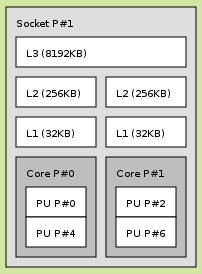
\includegraphics[scale=0.5]{img/caches.png}
\caption[Résultats]{Exemple d'une représentation des caches et des coeurs produit par lstopo}
\end{figure}


Pour la partie concernant les PCI il a fallut essayer plusieurs outils avec des résultats très variables. 

\begin{figure}[!h]
\centering
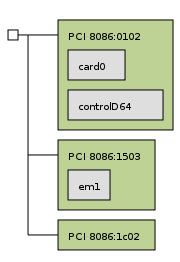
\includegraphics[scale=0.5]{img/treePCI.png}
\caption[Résultats]{Exemple d'un arbre PCI obtenu avec lstopo}
\end{figure}


Voici les principales technologies qui ont été testé pour se rapprocher au maximum d’un résultat satisfaisant :
\newline

\begin{itemize}
 \item La bibliothèque graphique javascript \textbf{D3.js} spécialisée dans la représentation de données sous forme graphique et dynamique.
 \item La bibliothèque javascript \textbf{JointJS} qui permet la création de diagramme interactif.
 \item Le composant HTML \textbf{canvas} qui permet la réalisation de dessin.
 \newline
\end{itemize}


Dans le cas de D3, en utilisant un modèle nativement destiné à la représentation d’arborescence de fichiers (collapsible indented tree) nous sommes parvenus à un résultat proche de celui attendu. La principale différence résidait dans la représentation des entités PCI qui n’était pas exactement la même.
\newline

Avec JointJS nous étions également parvenus à un résultat satisfaisant. Cette fois la différence se faisait dans la représentation des arêtes ou des branches qui n’étaient pas tout à fait conforme aux attentes.
\newline

Si les solutions avec ces deux outils ont été abandonnées, malgré le fait qu’elles permettaient une interaction, c’est parce que les deux différentes représentations que l’on obtenait était gravement déformées lors de l’exportation en PNG (une fonctionnalité importante de l’application). Tandis que les branches étaient transformées en polygone pleins, les entités étaient dépourvues de contour. 
\newline

Ces deux bibliothèques utilisent la technologie SVG (scalable vector graphics) pour la représentation des données. Or cela implique une conversion avec canvas avant de pouvoir être exporté sous un format d’image. C’est sans doute cette conversion qui posait problème mais n’ayant pas trouvé de véritable solution nous nous sommes tournée vers la troisième technologie : canvas.
\newline

Canvas est un composant qui fait partie de la spécification HTML5 et qui correspond à une zone de dessin. Du code javascript permet ensuite d’accéder à cette zone et d’utiliser toute une série de fonction de dessin comme une API classique.
\newline

L’interface graphique de l’application utilise l’outil \textbf{Bootstrap} et plusieurs directives AngularJS particulières :
\newline

\begin{itemize}
 \item \textbf{angular-bootstrap-colorpicker} pour une sélection poussée des couleurs sur chaque élément.
 \item \textbf{angular-multi-select} pour une liste déroulante des éléments à afficher ou non.
 \newline
\end{itemize}


La conversion du fichier XML en JSON pour une manipulation des données en JavaScript est possible grâce à la bibliothèque \textbf{x2js} qui à l’intérêt de ne pas avoir de dépendances.
\newline

\subsection{Fonctionnalités}

Pendant l'ensemble du projet nous avons réalisé les deux principales fonctionnalités demandées par le client qui sont : \newline

\begin{itemize}
\item La visualisation du fichier xml généré par hwloc pour tous les exemples possibles avec les éléments de base. Elle reprend exactement la représentation que fournissait Hwloc avec l'image produite par celui-ci. Effectivement le but n'était pas d'avoir une représentation différente de celle produite par hwloc mais d'avoir la même en web. Elle est réalisée essentiellement en html/css/Javascript avec utilisation de bordure pour faire les contours de chaque objet. 

\begin{figure}[!h]
\centering
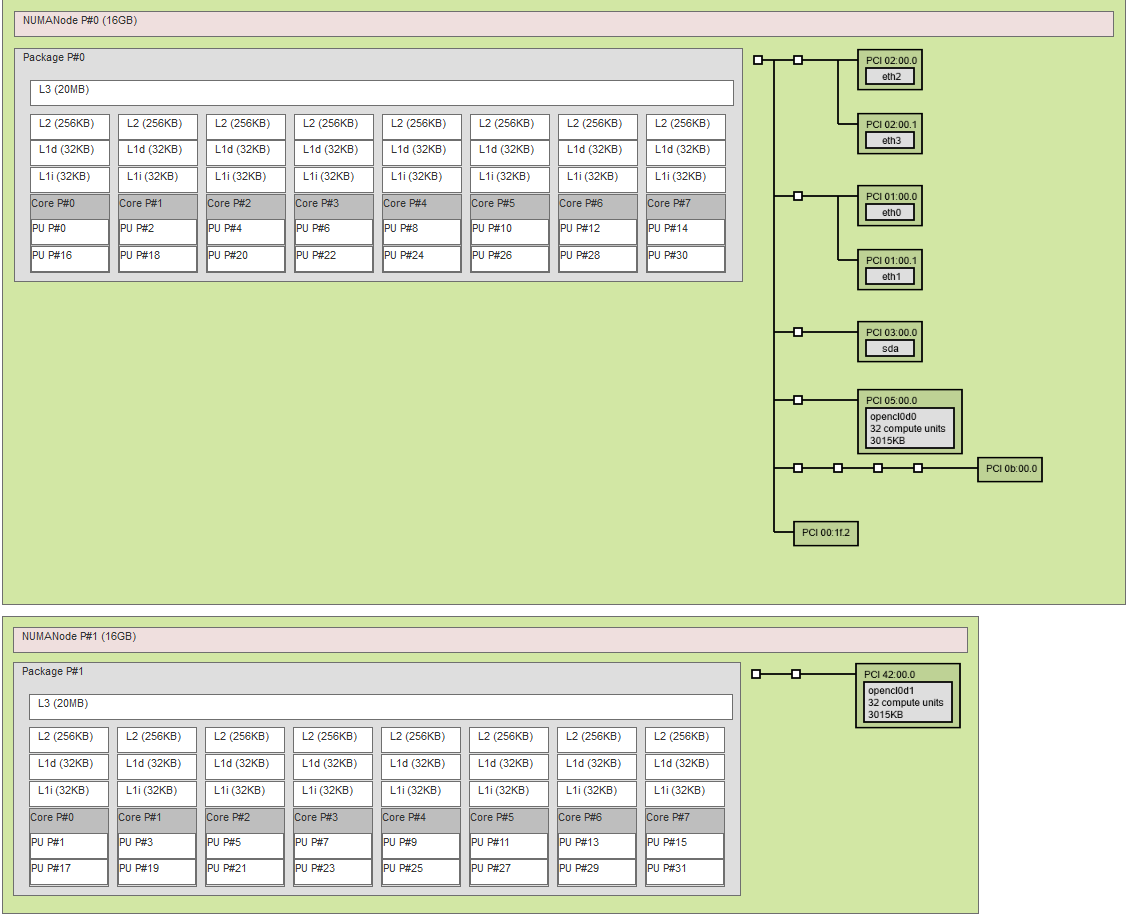
\includegraphics[scale=0.5]{img/alaric.png}
\caption[Résultats]{Exemple de représentation pour le xml Alaric}
\end{figure}

\item La seconde partie consistait à implémenter les options permettant de personnalisé l'affichage du fichier xml généré au besoin du client. Il contient : \newline
- la possibilité de cacher ou rendre visible certains éléments de la représentation comme les différents caches, la partie PCI ou des plus grosses entités comme des packages, groupes ou autres pour avoir une représentation spécifique ou plus générale. \newline
- une personnalisation des couleurs pour l'ensemble des objets selon les besoins des clients ou des standards mis en place. \newline
- changer la taille de police de caractère pour avoir un affichage plus ou moins gros selon la visibilité de base. \newline
- exporter au format PDF ou PNG l'ensemble des représentations personnalisées par le client.
- pour finir la possibilité d'enregistré sur notre machine la configuration des couleurs pour pouvoir la réutiliser plus tard et bien sur la possibilité de charger une configuration existante.


\begin{figure}[!h]
\centering
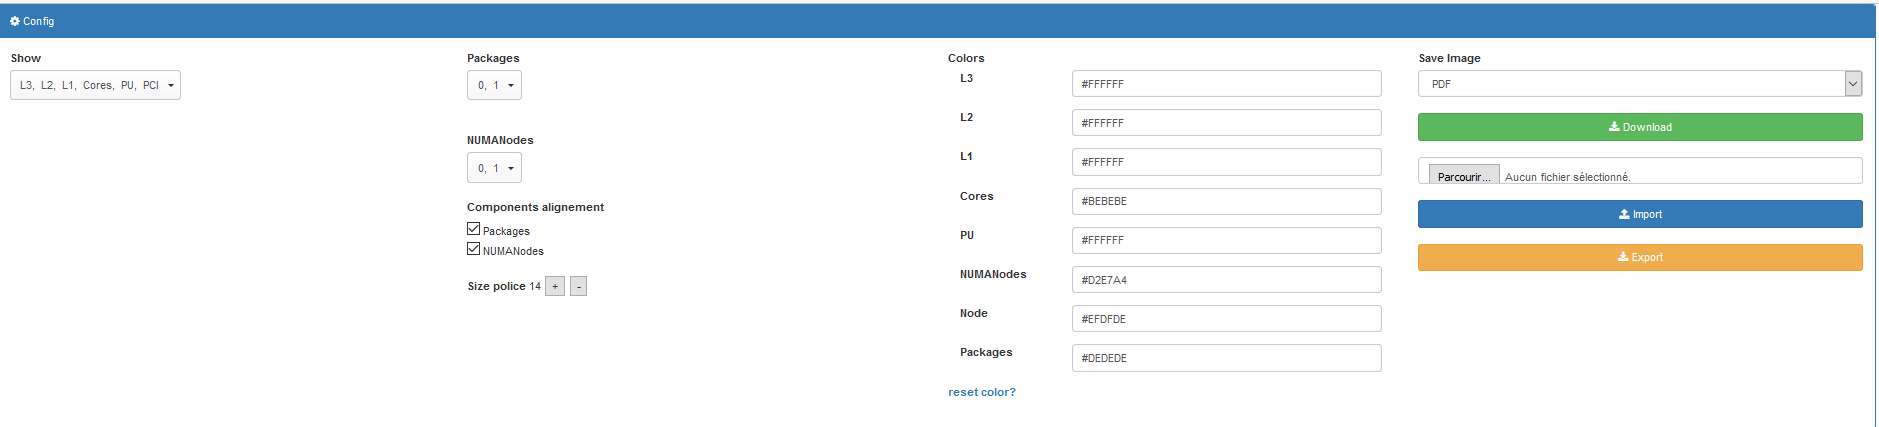
\includegraphics[scale=0.3]{img/filtre.png}
\caption[Résultats]{ Interface graphique du menu d'option }
\end{figure}

\begin{figure}[!h]
\centering
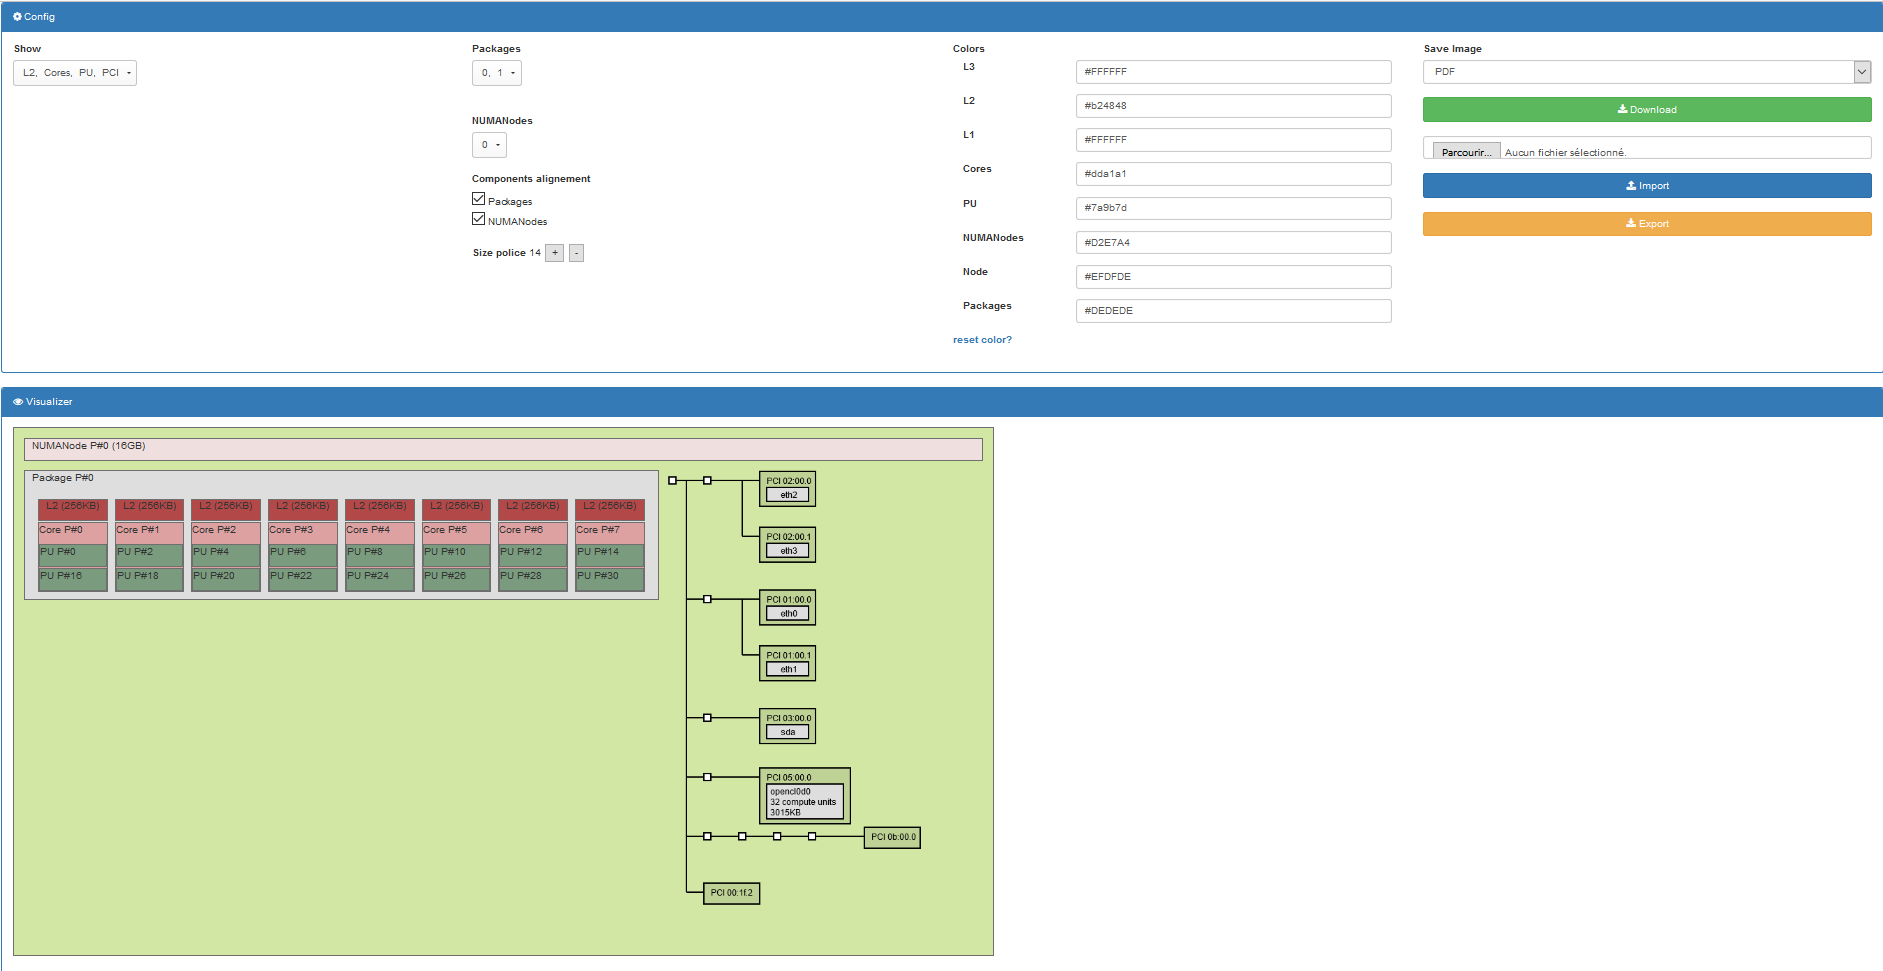
\includegraphics[scale=0.3]{img/alaric_modif.png}
\caption[Résultats]{Exemple de représentation pour le xml Alaric avec options}
\end{figure}

\end{itemize}

\newpage

\section{Intégration Continue}

Intégration continue est une étape importante à mettre en place dans le processus de développement logiciel. Nous parlerons donc ici de cette pratique et de l'outil utilisé au cours de ce projet.

\begin{center}
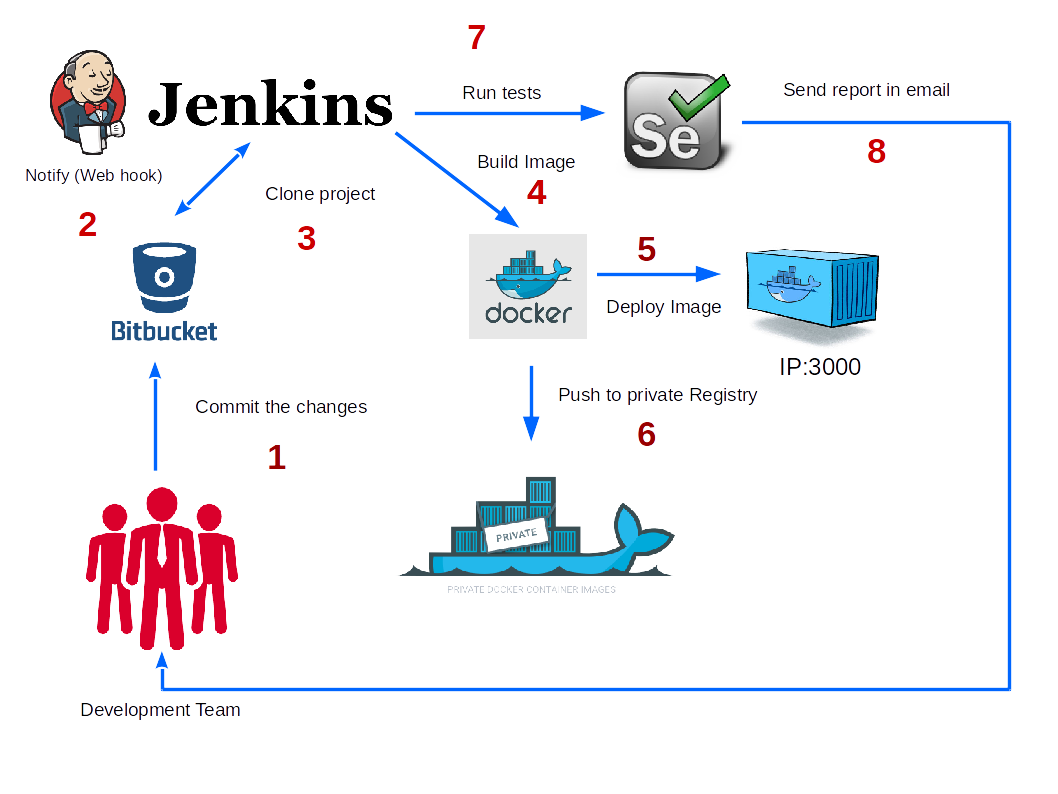
\includegraphics[scale=0.5]{img/ci.png}
\end{center}

Au moment d’un push d’un ou plusieurs commit au niveau de Bitbucket (sur la banche \textbf{release}) on déclenche via un hook la tâche de build qui permet la construction de l'image Docker à partir de Dockerfile, le push de cette image dans un dépot privé, le déploiement de cette image dans un container exposer sur le port 80 et enfin de passage des TUs au niveau de Jenkins. Dès qu’une modification du code est donc poussée sur le repository, il y a vérification que l’ensemble fonctionne toujours.

\begin{center}
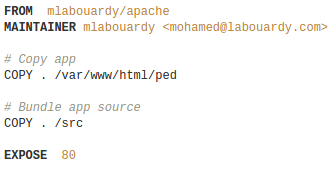
\includegraphics[scale=0.7]{img/Dockerfile.png}
\end{center}

\subsection{Bitbucket}

Un système de versionnement, il a été choisi pour héberger les sources des projets internes et clients.\cite{BITBUCKET} Pour notre projet on a utilisé 3 branches:\newline

\begin{itemize}
 \item \textbf{master} utilisé pour la phase de développement
 \item \textbf{release} utilisé pour la phase de production
 \item \textbf{docs} utilisé pour les documents (rapport, maquettes, cadrage ...)
\end{itemize}

\subsection{Jenkins}

Serveur d'intégration continue, il est capable d’aller se connecter à un outil de gestion de sources (Dans ce cas Git) et de voir si des modifications ont été effectuées. S’il en détecte, il peut lancer un \textbf{build} qui va pouvoir lancer un certain nombre d’actions(déploiement automatisé, tests unitaires ...)

\subsection{Docker}

Docker est un système de container linux ultra léger basé sur les cgroups, lxc et aufs.\newline

L'idée est la suivante pour un build:\newline

\begin{itemize}
 \item Jenkins crée une image docker à partir de Dockerfile
 \item Jenkins push l'image dans un dépot privé
 \item Jenkins crée un container docker à partir de cette image\newline
\end{itemize}

Les containers sont running de manière continue, permettant ainsi aux responsables du projet et au client de tester la dernière version du produit poussé manuellement à partir de Jenkins.

\subsection{Private Registry}

Depot pour stocker l'ensemble des versions de l'application tout au long de la phase de développement

\begin{center}
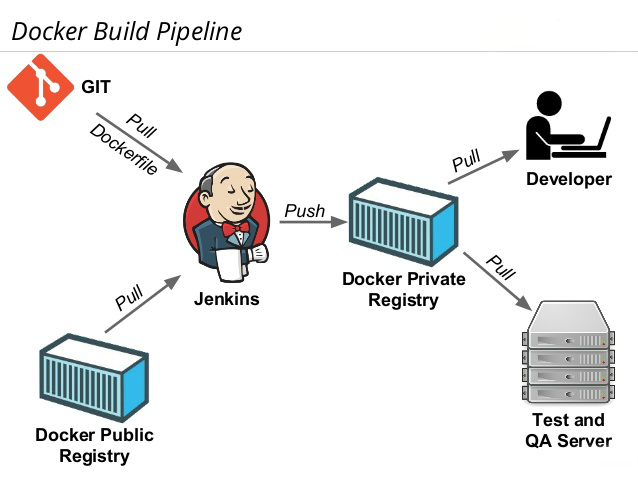
\includegraphics[scale=0.4]{img/registry.png}
\end{center}

L'avatange d'utilisation d'un docker private registry c'est avoir un systéme de versionning pour l'application. et rendre disponible facilement le dernier exécutable.
\subsection{Selenium Webdriver}
WebDriver est un framework de tests fonctionnels issu du projet Selenium, célèbre outil d'automatisation de tests pour navigateurs.\newline

Un exemple des test faites avec l'API Selenium c'est la mesure du temps d'execution pour un ensemble des exemples d'Architecture.

\begin{center}
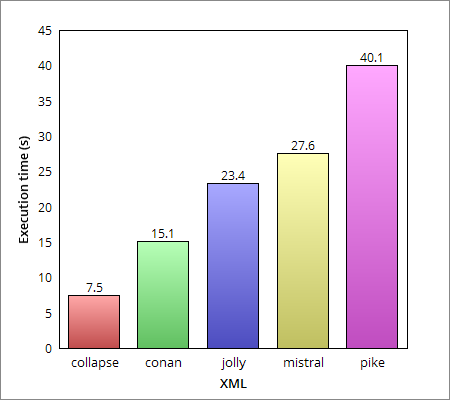
\includegraphics[scale=0.4]{img/benchmark.png}
\end{center}

\subsection{JSLint/CSSLint}

La qualité du code est vitale pour qu'un projet soit pérenne sur le moyen et long terme. De nombreux outils existent pour automatiser les contrôles et générer des rapports statistiques:\newline

\textbf{JSLint} est un analyseur de code Javascript. Son but est de parser le code Javascript pour vérifier que vous respecter les règles de coding Javascript.\newline

\begin{center}
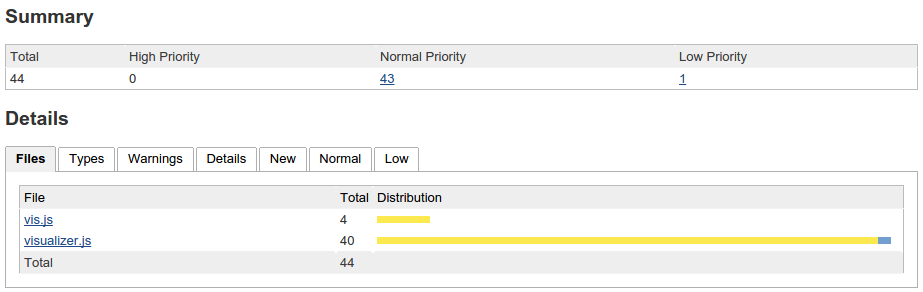
\includegraphics[scale=0.4]{img/checkstyle.png}
\end{center}

\textbf{CSSLint} détecte les problèmes d'une feuille de style CSS.

\begin{center}
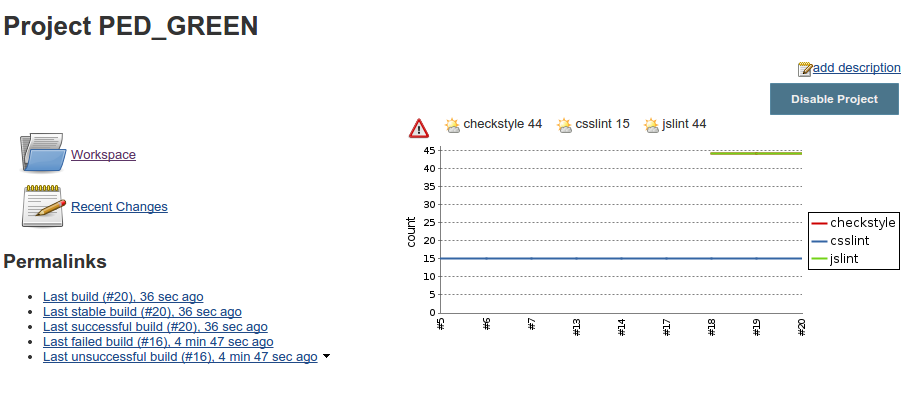
\includegraphics[scale=0.4]{img/jslint.png}
\end{center}

\subsection{AngularJS Batarang}

Afin de développer tester, déboguer et surveiller notre application AngularJS, on a installé un plugin sur le navigateur:\newline

Une extension de Google Chrome. Il permet d'observer le code en action, de faire des benchmarks sur les fonctions, modules, etc...

\newpage
\section{Gestion de projet}

\subsection{Scrum}

Durant l'ensemble du projet nous avons suivi la méthode Scrum qui est une méthode agile. Le but était d'être en conditions réelles de projet avec une équipe de 7 personnes. Pour appliquer la méthode Scrum on a utilisé le logiciel Icescrum qui permet de répondre aux besoins de ce genre de projet. Il nous a permis notamment de définir un backlog qui contenait l'ensemble des User Stories à faire pendant la durée du projet, définir différents sprints avec les User Stories à réaliser et les différentes taches de celles-ci. Dans chaque sprint on peut définir le kanban pour les différentes tâches et connaitre l'évolution de leurs taches. Nous avons choisi de réaliser des sprints de deux semaines comme c'était prévu à la base. 
Pour les taches nous avons choisi différentes couleurs afin de différencier les différents groupes de taches.\cite{ICESCRUM} Il y a :
\begin{itemize}
\item Taches jaune : Elles représentent le code produit pour le projet.
\item Taches bleu : Elles représentent les tests de validations pour notre code.
\item Taches grise : Elles représentent les tests d'intégrations.
\item Taches rouges : Elles représentent les recherches concernant certaines bibliothèques non mis en place mais qui peuvent améliorer le projet et le rapport.
\end{itemize}

\begin{figure}[!h]
\centering
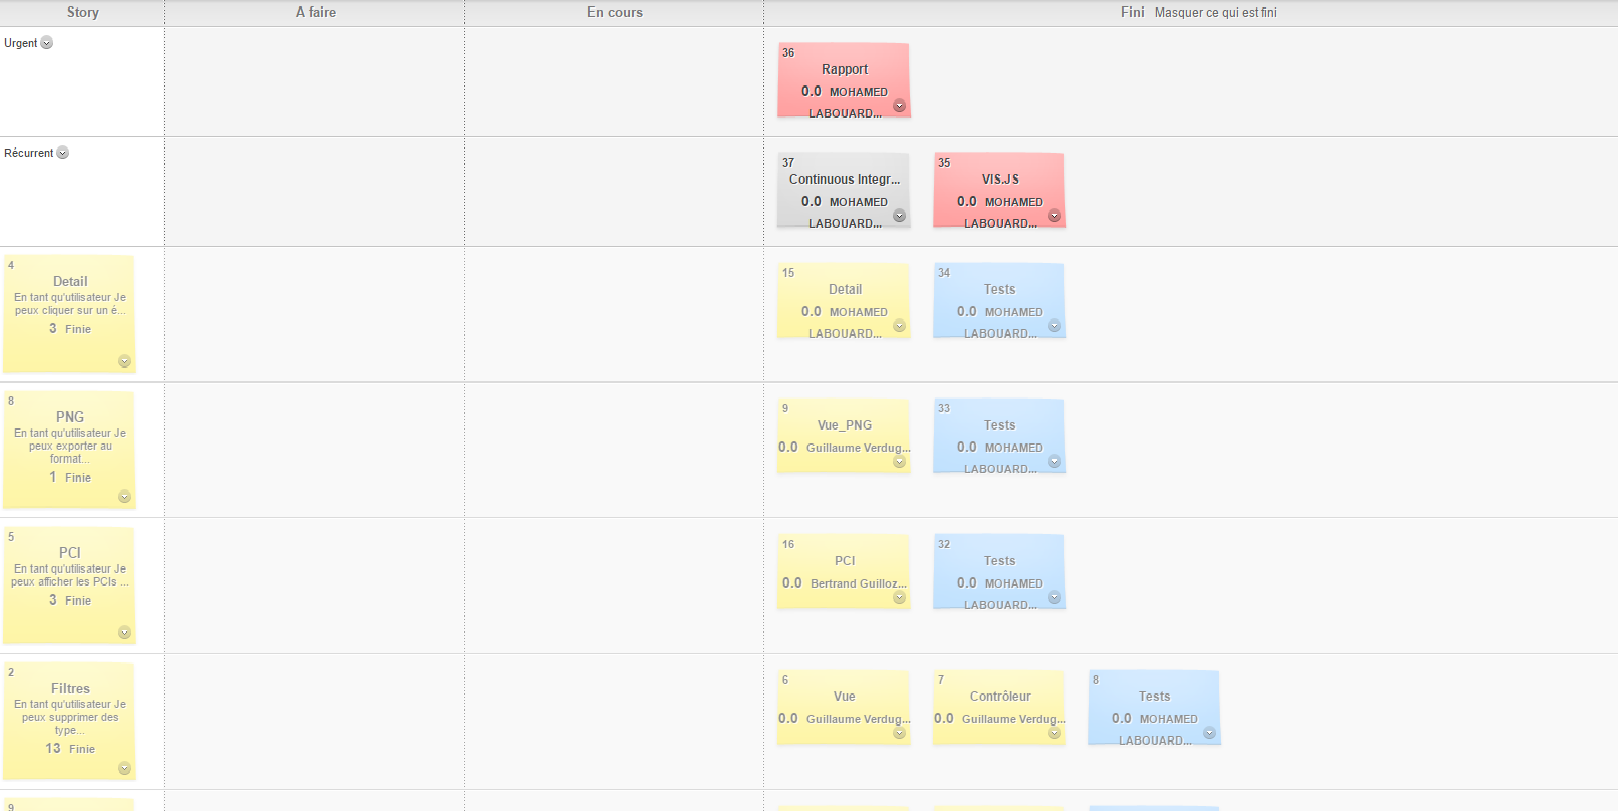
\includegraphics[scale=0.3]{img/icescrum.png}
\caption[Scrum]{ Sprint 2 avec les différentes taches }
\end{figure}

Par la suite on peut regarder l'évolution du projet avec le burn down chart qui est disponible pour chaque projet et via différent onglet voir les US fini et l'état des sprints.

\subsection{Outils complémentaires}

\newpage

\newpage

\section{Critiques}

\subsection{Technologies}
En ce qui concerne les technologies utilisées dans ce projet, on aurait pu utiliser reactjs qui est une bibliothèque développée par Facebook et permet de manipuler un DOM viruel. Et puisqu’on n’avait pas d’expériences avec cette bibliothèque, on a choisi de travailler avec angularjs.
\subsection{IceScrum}
Ce logiciel qui nous a été proposé durant le cycle de développement du projet et qu’on a due l’implémenter pour la gestion des taches au niveau des équipes était plus ou moins efficace à cause de sa lenteur et le temps mis pour la compréhension et l’adaptation avec notre besoin.


\subsection{Performances}
On peut trouver plusieurs pratiques qui peuvent nous permettre d’améliorer les performances de l’application, par exemple :\newline
-	L’utilisation du cache du navigateur qui consiste à garder en mémoire des copies des pages servies. Cela permettra d’éviter la répétition des traitements à chaque fois et gagner au niveau du temps du chargement de la page web.\newline
-	Le One time binding ( ::value) qui permet d’indiquer que le binding ne se fasse qu’une seule fois afin de gagner au niveau performance.
\subsection{Améliorations possibles}
En plus des améliorations citées bien avant, on peut aussi ajouter d’autres propositions possibles, notamment : \newline
-	Avoir une application responsive, c’est-à-dire offrir plus de réactivité à l’application afin qu’elle s’adapte aux différentes résolutions d’écrans disponibles.


\newpage

\nocite{*}
\bibliographystyle{plain}
\bibliography{report}




\end{document}
